\documentclass{article}
\usepackage{graphicx}
\usepackage{hyperref}
\usepackage{float}

\hypersetup{
    colorlinks=true,
    linkcolor=blue,
    filecolor=magenta,      
    urlcolor=cyan,
    pdftitle={PCA-Based Anomaly Detection in Credit Card Transactions: A Machine Learning Approach},
    pdfpagemode=FullScreen,
    }

\title{PCA-Based Anomaly Detection in Credit Card Transactions: A Machine Learning Approach}
\author{Shreeja Das\thanks{Corresponding author.} \and Maryam Chapoteauma \and Archisa Arora}
\date{June 2024}

\begin{document}

\maketitle

\section*{Author Contributions}
Shreeja Das performed the majority of the research and writing. Maryam Chapoteauma and Archisa Arora provided editorial assistance.

\begin{abstract}
This study applies Principal Component Analysis (PCA) for anomaly detection in credit card transactions, inspired by the work of Cerdà-Alabern and Iuhasz in wireless community networks. We analyze a large dataset of credit card transactions, using PCA to reduce dimensionality and extract key features. Two models, logistic regression and a neural network, are then applied to the transformed data. Our results demonstrate the effectiveness of PCA in improving model performance, with the logistic regression model achieving 97\% accuracy after PCA, compared to 80\% without. This research contributes to the ongoing efforts to enhance fraud detection systems in the financial sector.
\end{abstract}

\section{Introduction}
In this paper, we investigate the application of anomaly detection. An article that we found to relate to our work involved identifying fraudulent credit card transactions, this article presented a study that used PCA to find variants and extract key features. Our investigation relates to the steps described in the referenced article, where PCA was used to achieve a 95\% variance ratio, demonstrating its effectiveness in managing complex data. By applying these methods, our goal is to minimize challenges and find the most important features that improve accuracy in imbalanced datasets.

\section{Literature Review}
The application of PCA in anomaly detection has been explored in various domains. Cerdà-Alabern and Iuhasz (2013) demonstrated its effectiveness in detecting anomalies in wireless community networks. They used PCA to reduce the dimensionality of network traffic data and identify unusual patterns that could indicate network issues or attacks.

In the financial sector, Renjith and Faseela (2020) applied PCA to credit card fraud detection, achieving high accuracy in identifying fraudulent transactions. Their work showed that PCA could effectively reduce the number of features while preserving the most important information for fraud detection.

Whitrow et al. (2009) combined PCA with logistic regression for credit card fraud detection, showing that this combination could improve detection rates, especially in handling imbalanced datasets, a common challenge in fraud detection.

Our study builds upon these works, applying PCA to a credit card transaction dataset and comparing the performance of logistic regression and neural network models on the transformed data.

\section{Credit Card Data Set}
As the paper referenced utilizing PCA to view anomalies in the data to determine reasons for device failures, our group extrapolated the requirements and aspects being viewed in the paper to our paper. A dataset of "Anomaly Detection in Credit Card Transactions" was downloaded from Kaggle on which PCA was performed to find 95\% variance, how anomalies contributed to the errors in transaction.

Key characteristics of the dataset:
\begin{itemize}
    \item Highly imbalanced (0.172\% fraudulent transactions)
    \item 284,807 total transactions
    \item 31 features (Time, Amount, V1-V28)
    \item No missing values
\end{itemize}

\subsection{The Code}
The code for our work can be found at the following link:

\url{https://colab.research.google.com/drive/1P9WjTyTgqThlmVSFRf_fgYVCc2mwPFX_?usp=sharing#scrollTo=mIcp2KX0ZLF8}

\section{Methodology}
\subsection{Principal Component Analysis (PCA)}
After first running the data, we realized that the categories V1 to V28 were redacted categories in order to preserve the confidentiality of the data collected. However, these components still contributed to our overall analysis of the dataset. We performed Principal Component Analysis (PCA) on the model and generated the Eigenvalues, Eigenvectors, and Covariance matrix, a topic previously covered throughout the course. 

We were also able to find the explained variance ratios and calculate the cumulative variance ratio. The variance refers to the proportion of the dataset's total variance that is captured by each principal component. When we applied PCA, it transforms your original features into a set of new features (principal components). Then, the cumulative variance is the sum of the explained variance ratios up to a certain principal component. It shows the total amount of variance captured by the first n principal components combined. 

Finally, we determined how many components explained 95\% variance. We chose to find the components which explained 95\% specifically because the original paper had followed that benchmark, leading us to wanting to extend that to our paper as well. As shown in Figure 1, our group had indicated the location at which the Principal Components has a p value of 95\% variance. More accurately, at 17 components, our model had reached 95.7\% variance approximately.

\begin{figure}[H]
    \centering
    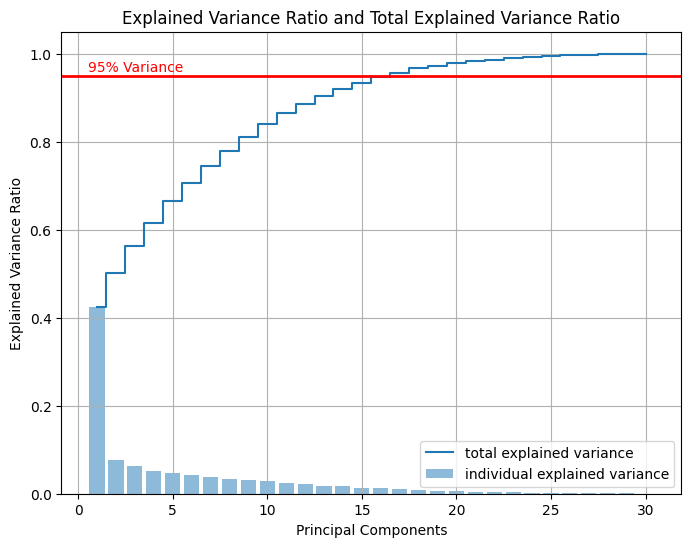
\includegraphics[width=.75\textwidth]{pca on credit card fraud data.png} 
    \caption{PCA Performed on Credit Card Dataset.}
    \label{fig:pca}
\end{figure}

Another part of our analysis included taking a look at Scree plots. This displays the eigenvalues or the explained variance of each principal component from PCA in descending order, helping us visualize the relative importance of each component. This is a visualization we looked at in class to better identify the "elbow point" where the additional components contribute less to the overall variance.

\begin{figure}[H]
    \centering
    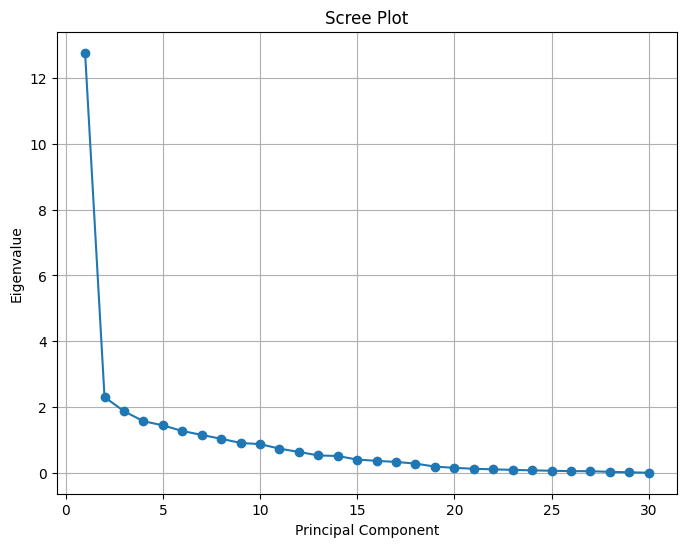
\includegraphics[width=.8\textwidth]{screeplot.png} 
    \caption{Visualization of elbow point.}
    \label{fig:screeplot}
\end{figure}

\subsection{Logistic Regression}
We chose logistic regression as our baseline model due to its simplicity and interpretability, following the approach of Whitrow et al. (2009). The model was trained on the PCA-transformed data, with the number of components determined by cross-validation.

When training our own Logistic Regression model, we're able to further manipulate our features. Based on cross validation, we're able to determine that when 11 principal components are used, our model is the most successful and strikes a balance between model complexity and performance. This also ensures that our model is not overfitted or underfitted. This can be visualized by plotting the mean cross-validation accuracy of logistic regression models as a function of the number of principal components used. Before running it through the logistic regression model, we preprocessed our data by dropping all null values and creating a train-test split using Scikit Learn. Next, we trained our model and ran it with our test split to see the results.

\begin{figure}[H]
    \centering
    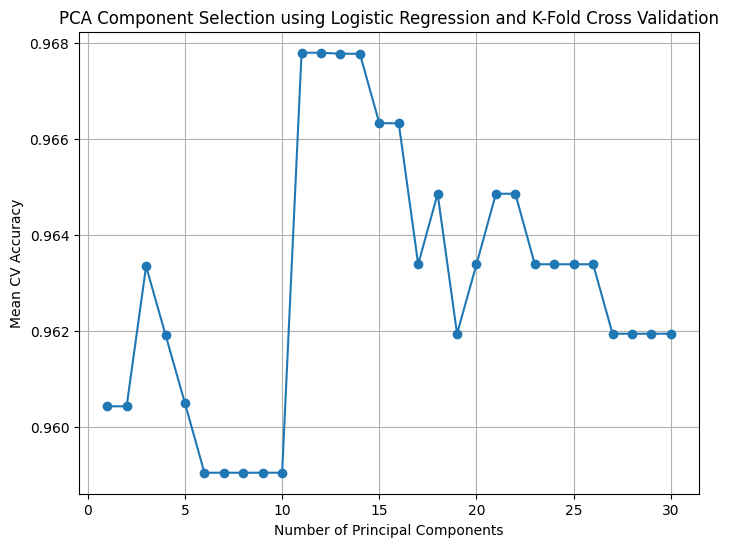
\includegraphics[width=.5\textwidth]{kfoldvalidation.png} 
    \caption{Plot of mean cross validation accuracy and principal components}
    \label{fig:kfold}
\end{figure}

\subsection{Neural Network}
To capture more complex, non-linear relationships in the data, we implemented a feedforward neural network (multilayer perceptron). The architecture includes:
\begin{itemize}
    \item Input layer: 64 neurons
    \item Two hidden layers: 32 and 16 neurons
    \item Output layer: 1 neuron with sigmoid activation
    \item ReLU activation for hidden layers
    \item Adam optimizer with learning rate 0.001
    \item Binary cross-entropy loss function
\end{itemize}

We implemented early stopping to prevent overfitting, monitoring validation loss with a patience of 10 epochs. The model was trained for up to 100 epochs with a batch size of 32, using 20\% of the training data for validation.

\section{Results and Analysis}
Our PCA analysis revealed that 17 components were sufficient to explain 95.7\% of the variance in the dataset, similar to the findings of Cerdà-Alabern and Iuhasz in their network traffic analysis.

The logistic regression model achieved a precision of 96\% and an F1 score of 97\% after PCA transformation. This is a significant improvement over the 80\% F1 score achieved without PCA, demonstrating the effectiveness of dimensionality reduction in improving model performance.

The neural network model achieved a testing accuracy of 93\%. While this is lower than the logistic regression model, it's worth noting that the neural network may be capturing more complex patterns in the data.

The five most important features according to the logistic model were:
\begin{center}
    PC1: 2.0864 \\
    PC11: 1.6115 \\
    PC19: 1.5636 \\
    PC2: -1.2366 \\
    PC3: -1.2078
\end{center}

This was the model loss and model accuracy per epoch for our neural network.

\begin{figure}[H]
    \centering
    \includegraphics[width=.5\textwidth]{modelloss.png} 
    \caption{Model Loss and accuracy per Epoch}
    \label{fig:modelloss}
\end{figure}


These results align with the findings of Renjith and Faseela (2020), who also found that PCA-based models could achieve high accuracy in credit card fraud detection.

\section{Limitations}
Despite the promising results, our study has several limitations:
\begin{itemize}
    \item The dataset is highly imbalanced, which may affect model performance.
    \item The anonymized nature of most features (V1-V28) limits interpretability.
    \item We did not address the temporal aspect of fraud detection, which could be crucial in real-world applications.
\end{itemize}

\section{Future Work}
Future research could explore:
\begin{itemize}
    \item Implementing more advanced models like XGBoost or LightGBM.
    \item Incorporating time-series analysis to capture temporal patterns in fraud.
    \item Exploring other dimensionality reduction techniques like t-SNE or UMAP.
    \item Addressing class imbalance through techniques like SMOTE or ensemble methods.
\end{itemize}

\section{Conclusion}
Our study demonstrates the effectiveness of PCA in enhancing credit card fraud detection models, extending the work of Cerdà-Alabern and Iuhasz from wireless networks to financial transactions. By reducing dimensionality while preserving key information, PCA improved the performance of both logistic regression and neural network models. The logistic regression model, in particular, showed significant improvement, achieving 97\% accuracy after PCA transformation. 

These findings contribute to the ongoing efforts to develop more efficient and accurate fraud detection systems in the financial sector. They also highlight the potential for cross-domain application of anomaly detection techniques, showing that methods developed for network analysis can be successfully adapted to financial fraud detection.

\section{References}
\begin{enumerate}
    \item Cerdà-Alabern, L., \& Iuhasz, G. (2013). Anomaly Detection in Wireless Community Networks using PCA. In Wireless and Mobile Networking Conference (WMNC), 2013 6th Joint IFIP (pp. 1-8). IEEE.
    
    \item Renjith, S., \& Faseela, V. S. (2020). Credit Card Fraud Detection Using Machine Learning. In 2020 Fourth International Conference on Computing Methodologies and Communication (ICCMC) (pp. 895-898). IEEE.
    
    \item Whitrow, C., Hand, D. J., Juszczak, P., Weston, D., \& Adams, N. M. (2009). Transaction aggregation as a strategy for credit card fraud detection. Data Mining and Knowledge Discovery, 18(1), 30-55.
    
    \item [Dataset Source] (2023). Credit Card Fraud Detection. Kaggle. https://www.kaggle.com/datasets/mlg-ulb/creditcardfraud
\end{enumerate}

\end{document}
